\documentclass[../Tesi_Jiahao_Miao_986136.tex]{subfiles}
\begin{document}

\subsection{Renormalization-scale dependence} \label{subsec:Renormalization_scale_dependence}
In this section we consider renormalization-scale dependence of our results. In principle, such scale $\mu$ should not appear in
the cross sections, as it does not correspond to any fundamental constant or kinematical scale in the problem.
The completely resummed perturbative expansion of an observable is indeed formally independent on $\mu$.
In practise, truncated perturbative expansions exhibit a residual scale dependence, because of neglected higher orders.

We start with deriving the strong coupling $\alpha_s (Q^2)$ as a function of $\alpha_s(\mu^2)$ and $\mu^2/Q^2$, to do so we expand 
the explicit \cref{eq:N4LO} in powers of $\alpha_s(\mu^2)$ and obtain:

\begin{align}
    \begin{split}\label{eq:renormalization scale dependence}
        \alpha_s(Q^2) &= \alpha_s(\mu^2) + \alpha_s^2(\mu^2) b_0 \ln(\frac{\mu^2}{Q^2}) + \alpha_s^3(\mu^2) \biggl[b_1 \ln(\frac{\mu^2}{Q^2}) + b_0^2 \ln^2\qty(\frac{\mu^2}{Q^2})\biggr] \\
        &+ \alpha_s^4 (\mu^2) \biggl[ b_2 \ln(\frac{\mu^2}{Q^2}) + \frac{5}{2} b_0 b_1 \ln^2\qty(\frac{\mu^2}{Q^2}) + b_0^3 \ln^3\qty(\frac{\mu^2}{Q^2})\biggr] \\
        &+ \alpha_s^5(\mu^2) \biggl[ b_3 \ln(\frac{\mu^2}{Q^2}) + \qty(\frac{3}{2} b_1^2 + 3 b_0 b_2 ) \ln^2\qty(\frac{\mu^2}{Q^2}) \\
        &+ \frac{13}{3} b_0^2 b_1 \ln^3\qty(\frac{\mu^2}{Q^2}) + b_0^4 \ln^4\qty(\frac{\mu^2}{Q^2}) \biggr] + \order{\alpha_s^6(\mu^2)}.
    \end{split}
\end{align}

For brevity we'll write: 

\begin{equation}
    \alpha_s(Q^2) = \alpha_s(\mu^2) + c_1 \alpha_s^2(\mu^2) + c_2 \alpha_s^3(\mu^2) + c_3 \alpha_s^4(\mu^2) + c_4 \alpha_s^5(\mu^2) + \order{\alpha_s^6(\mu^2)},
\end{equation}

where $c_i$ are the coefficients of the expansion above.

\begin{flalign}
    \begin{split}
        c_1 &= b_0 \ln(\frac{\mu^2}{Q^2}), \\
        c_2 &= b_1 \ln(\frac{\mu^2}{Q^2}) + b_0^2 \ln^2\qty(\frac{\mu^2}{Q^2}),\\
        c_3 &= b_2 \ln(\frac{\mu^2}{Q^2}) + \frac{5}{2} b_0 b_1 \ln^2\qty(\frac{\mu^2}{Q^2}) + b_0^3 \ln^3\qty(\frac{\mu^2}{Q^2}), \\
        c_4 &= b_3 \ln(\frac{\mu^2}{Q^2}) + \qty(\frac{3}{2} b_1^2 + 3 b_0 b_2 ) \ln^2\qty(\frac{\mu^2}{Q^2}) + \frac{13}{3} b_0^2 b_1 \ln^3\qty(\frac{\mu^2}{Q^2}) + b_0^4 \ln^4\qty(\frac{\mu^2}{Q^2}).
    \end{split}
\end{flalign}

Now we substitute \cref{eq:renormalization scale dependence} into $\lambda = b_0 \alpha_s(Q^2) L$ and obtain: 

\begin{equation}
    \lambda(Q^2) = \lambda(\mu^2) \qty(1 + c_1 \alpha_s(\mu^2) + c_2 \alpha_s^2(\mu^2) + c_3 \alpha_s^3(\mu^2) + c_4 \alpha_s^4(\mu^2) + \order{\alpha_s^5(\mu^2)} ),
\end{equation}

and formally expand in powers of $\alpha_s(\mu^2)$ all the relevant functions, now $\lambda = \lambda(\mu^2)$:

\begin{flalign}
        L f_1(Q^2) &= L f_1(\lambda) + \frac{c_1}{b_0} \lambda^2 f_1'(\lambda)  + \frac{\lambda}{b_0}\qty(c_2 \lambda f_1'(\lambda) + \frac{1}{2}c_1^2 \lambda^2 f_1''(\lambda)) \textcolor{red}{\alpha_s} \\
        &+ \frac{\lambda}{b_0}\qty(c_3 \lambda f_1'(\lambda) +c_1 c_2 \lambda^2 f_1''(\lambda) +\frac{1}{6}c_1^3 f_1^{(3)}(\lambda) ) \textcolor{blue}{\alpha_s^2} + \frac{\lambda^2}{b_0} \biggl(c_4 f_1'(\lambda) \nonumber\\
        &+ \frac{1}{2}c_2^2 \lambda f_1''(\lambda) + c_1 c_3 \lambda f_1''(\lambda) +  \frac{1}{2} c_1^2 c_2 \lambda^2 f_1^{(3)}(\lambda) + \frac{1}{24} c_1^4 \lambda^3 f_1^{(4)}(\lambda) \biggr) \textcolor{green}{\alpha_s^3}\nonumber ,\\
        f_2(Q^2) &=  f_2(\lambda) + c_1 \lambda f_2'(\lambda) \textcolor{red}{\alpha_s} +\qty(c_2 \lambda f_2'(\lambda) +\frac{1}{2}c_1^2\lambda^2 f_2''(\lambda)) \textcolor{blue}{\alpha_s^2} \\ 
        &+ \qty(c_3 \lambda f_2'(\lambda) + c_1 c_2 \lambda^2 f_2''(\lambda) + \frac{1}{6} c_1^3 f_2^{(3)}(\lambda)) \textcolor{green}{\alpha_s^3} ,\nonumber\\
        \textcolor{red}{\alpha_s}f_3(Q^2) &= \textcolor{red}{\alpha_s}f_3(\lambda)  + c_1 \lambda f_3'(\lambda) \textcolor{blue}{\alpha_s^2} + \qty(c_2 \lambda f_3'(\lambda) + \frac{1}{2} c_1^2 \lambda^2 f_3''(\lambda)) \textcolor{green}{\alpha_s^3}, \\
        \textcolor{blue}{\alpha_s^2}f_4(Q^2) &= \textcolor{blue}{\alpha_s^2}f_4(\lambda)  + c_1 \lambda f_4'(\lambda) \textcolor{green}{\alpha_s^3},\\
        \textcolor{green}{\alpha_s^3}f_5(Q^2) &= \textcolor{green}{\alpha_s^3}f_5(\lambda) .
\end{flalign}

As usual, the terms from the expansion proportional to $\textcolor{red}{\alpha_s}$ corrects $f_3$, the terms proportional to $\textcolor{blue}{\alpha_s^2}$ corrects $f_4$ and so on. 

So the additional terms in the functions $f_i$, to partially compensate for the scale change $Q^2\to \mu^2$, read:

\begin{flalign}
        \delta f_1\qty(\lambda,\frac{\mu^2}{Q^2}) &= 0 ,\\
        \delta f_2\qty(\lambda,\frac{\mu^2}{Q^2}) &=  \lambda^2 f_1'(\lambda) \log \frac{\mu^2}{Q^2} ,\\ 
        \delta f_3\qty(\lambda,\frac{\mu^2}{Q^2}) &= \frac{1}{2} b_0 \lambda ^3 f_1''(\lambda ) \log ^2\frac{\mu ^2}{Q^2}+\lambda ^2 \left(b_0 f_1'(\lambda ) \log ^2\frac{\mu ^2}{Q^2}+\frac{b_1}{b_0} f_1'(\lambda ) \log \frac{\mu ^2}{Q^2}\right)\\
        &+b_0 \lambda  f_2'(\lambda ) \log \frac{\mu ^2}{Q^2},\nonumber\\
        \delta f_4\qty(\lambda,\frac{\mu^2}{Q^2}) &= \frac{1}{6} b_0^2 \lambda ^4 f_1{}^{(3)}(\lambda ) \log ^3\frac{\mu ^2}{Q^2}+\lambda ^3 \left(b_0^2 f_1''(\lambda ) \log ^3\frac{\mu ^2}{Q^2}+b_1 f_1''(\lambda ) \log ^2\frac{\mu ^2}{Q^2}\right)\\
        &+\lambda ^2 \left(b_0^2 f_1'(\lambda ) \log ^3\frac{\mu ^2}{Q^2}+\frac{5}{2} b_1 f_1'(\lambda ) \log ^2\frac{\mu ^2}{Q^2}+\frac{b_2}{b_0} f_1'(\lambda ) \log \frac{\mu ^2}{Q^2}+\frac{1}{2} b_0^2 f_2''(\lambda ) \log ^2\frac{\mu ^2}{Q^2}\right)\nonumber\\
        &+\lambda  \left(b_0^2 f_2'(\lambda ) \log ^2\frac{\mu ^2}{Q^2}+b_0 f_3'(\lambda ) \log \frac{\mu ^2}{Q^2}+b_1 f_2'(\lambda ) \log \frac{\mu ^2}{Q^2}\right),\nonumber\\
        \delta f_5\qty(\lambda,\frac{\mu^2}{Q^2}) &= \frac{1}{24} b_0^3 \lambda ^5 f_1{}^{(4)}(\lambda ) \log ^4\frac{\mu ^2}{Q^2}+\lambda ^4 \biggl(\frac{1}{2} b_0^3 f_1{}^{(3)}(\lambda ) \log ^4\frac{\mu ^2}{Q^2}\\
        &+\frac{1}{2} b_0 b_1 f_1{}^{(3)}(\lambda ) \log ^3\frac{\mu ^2}{Q^2}\biggr)+\lambda ^3 \biggl(\frac{3}{2} b_0^3 f_1''(\lambda ) \log ^4\frac{\mu ^2}{Q^2}+\frac{7}{2} b_0 b_1 f_1''(\lambda ) \log ^3\frac{\mu ^2}{Q^2}\nonumber\\
        &+\frac{b_1^2}{2 b_0} f_1''(\lambda ) \log ^2\frac{\mu ^2}{Q^2}+b_2 f_1''(\lambda ) \log ^2\frac{\mu ^2}{Q^2}+\frac{1}{6} b_0^3 f_2{}^{(3)}(\lambda ) \log ^3\frac{\mu ^2}{Q^2}\biggr)\nonumber\\
        &+\lambda ^2 \biggl(b_0^3 f_1'(\lambda ) \log ^4\frac{\mu ^2}{Q^2}+\frac{13}{3} b_0 b_1 f_1'(\lambda ) \log ^3\frac{\mu ^2}{Q^2}+\frac{3 b_1^2}{2 b_0} f_1'(\lambda ) \log ^2\frac{\mu ^2}{Q^2}\nonumber\\
        &+3 b_2 f_1'(\lambda ) \log ^2\frac{\mu ^2}{Q^2}+\frac{b_3}{b_0} f_1'(\lambda ) \log \frac{\mu ^2}{Q^2}+b_0^3 f_2''(\lambda ) \log ^3\frac{\mu ^2}{Q^2}+b_0 b_1 f_2''(\lambda ) \log ^2\frac{\mu ^2}{Q^2}\nonumber\\
        &+\frac{1}{2} b_0^2 f_3''(\lambda ) \log ^2\frac{\mu ^2}{Q^2}\biggr) +\lambda  \biggl(b_0^3 f_2'(\lambda ) \log ^3\frac{\mu ^2}{Q^2}+b_0^2 f_3'(\lambda ) \log ^2\frac{\mu ^2}{Q^2}\nonumber\\
        &+\frac{5}{2} b_1 b_0 f_2'(\lambda ) \log ^2\frac{\mu ^2}{Q^2}+b_0 f_4'(\lambda ) \log \frac{\mu ^2}{Q^2}+b_2 f_2'(\lambda ) \log \frac{\mu ^2}{Q^2}+b_1 f_3'(\lambda ) \log \frac{\mu ^2}{Q^2}\biggr).\nonumber
\end{flalign}

By varying the renormalization scale $\mu$ in the range $Q/2 \leq \mu \leq 2Q$, where $Q = m_Z$ we can estimate the uncertainty due to the truncation of the perturbative expansion.

\begin{figure}[h!]
    \centering
    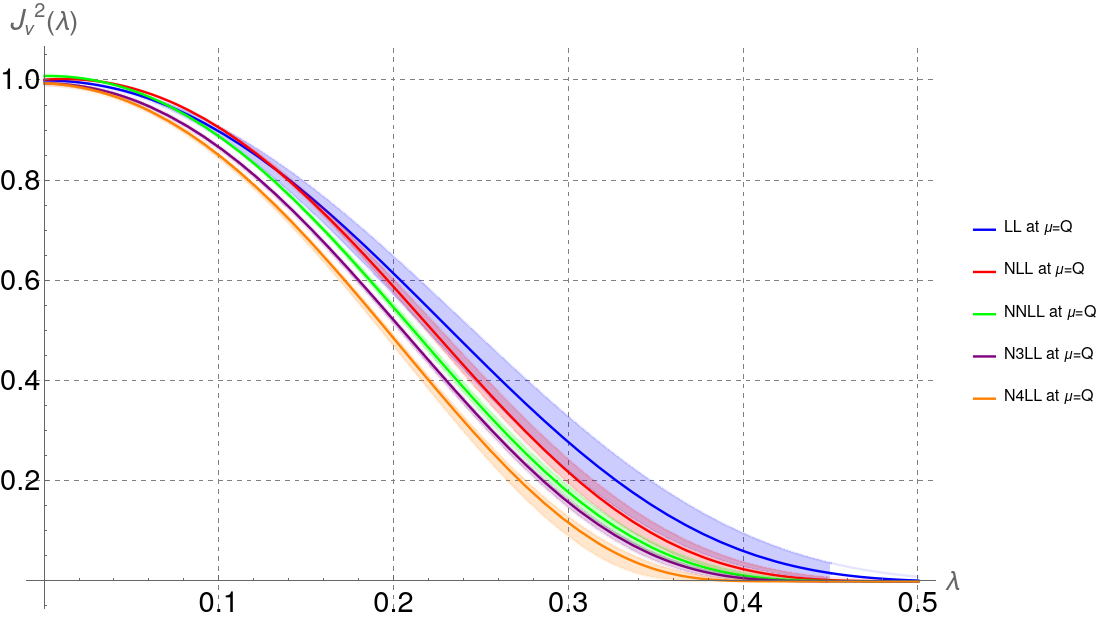
\includegraphics[width=0.6\textwidth]{figures/scale_variation_all.png}
    \caption{Plot of $J_\nu ^2$ \cref{eq:factorized_J_nu}. Dependence on renormalization scale $\mu$ for LL, NLL, NNLL, N$^3$LL and N$^3$LL logarithmic accuracy.}
    \label{fig:renormalization_scale_dependence}
\end{figure}

\begin{figure}[h!]
    \centering
    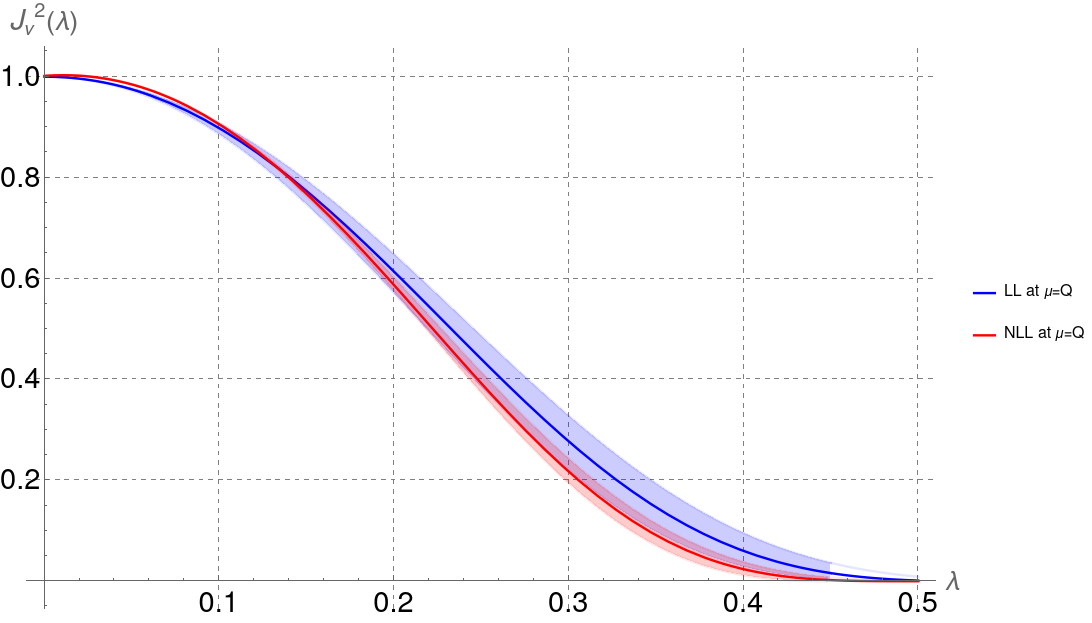
\includegraphics[width=0.6\textwidth]{figures/scale_variation_LL-NLL.png}
    \caption{Scale variation of the Laplace transformed Thrust distribution \cref{eq:factorized_J_nu} for Leading Logarithm and Next-to-Leading Logarithm accuracy.}
\end{figure}
\begin{figure}[h!]
    \centering
    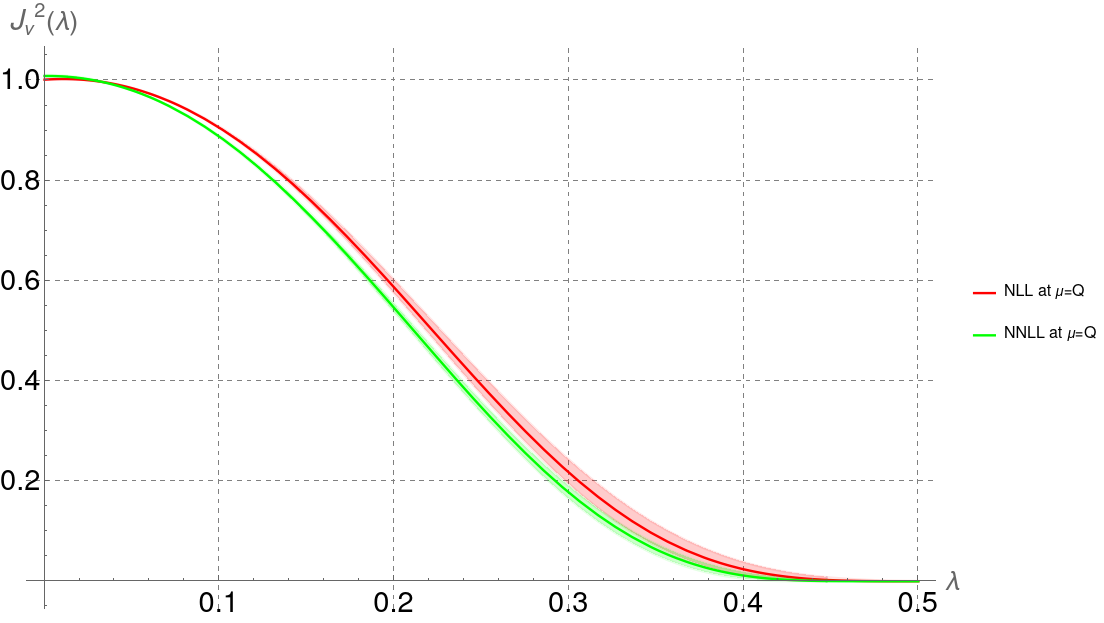
\includegraphics[width=0.6\textwidth]{figures/scale_variation_NLL-NNLL.png}
    \caption{Scale variation of the Laplace transformed Thrust distribution \cref{eq:factorized_J_nu} for NLL and NNLL.}
\end{figure}
\begin{figure}[h!]
    \centering
    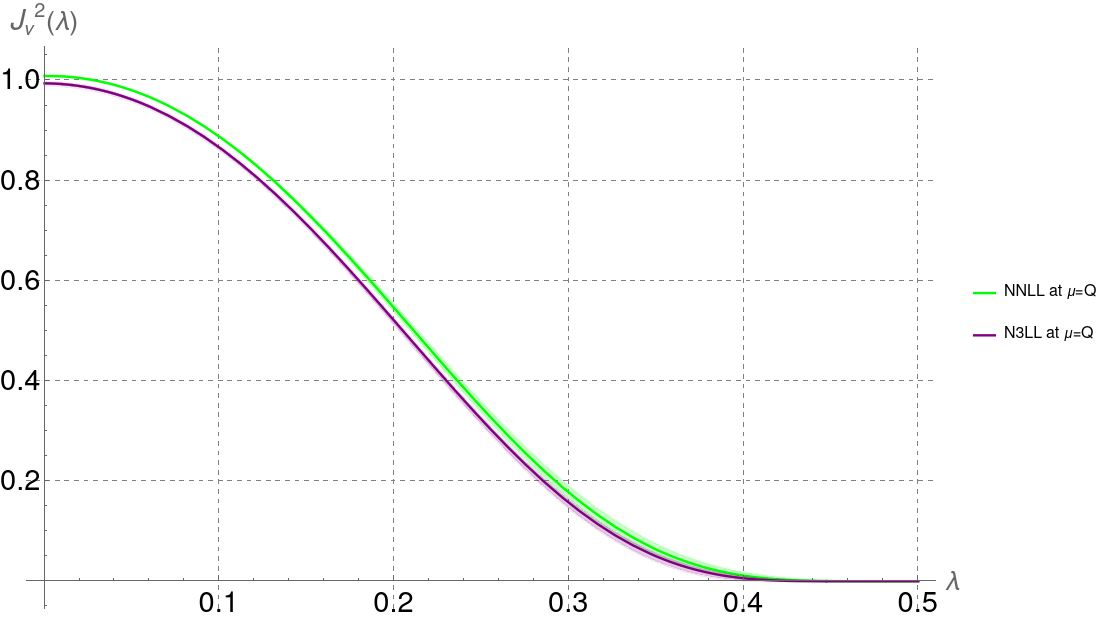
\includegraphics[width=0.6\textwidth]{figures/scale_variation_NNLL-N3LL.png}
    \caption{Scale variation of the Laplace transformed Thrust distribution \cref{eq:factorized_J_nu} for NNLL and N$^3$LL.}
\end{figure}
\begin{figure}[h!]
    \centering
    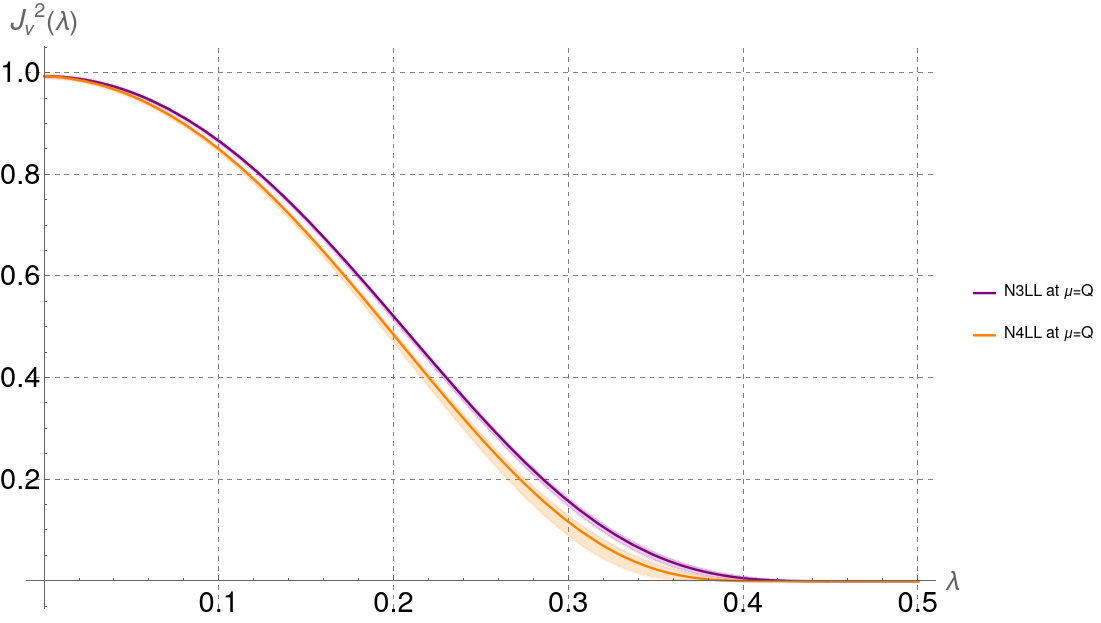
\includegraphics[width=0.6\textwidth]{figures/scale_variation_N3LL-N4LL.png}
    \caption{Scale variation of the Laplace transformed Thrust distribution \cref{eq:factorized_J_nu} for N$^3$LL and N$^4$LL.}
\end{figure}

We observe how the scale dependence decreases as we increase the logarithmic accuracy of the resummation. The N$^3$LL result is the most stable under scale variations,
while N$^4$LL has some anomalous behavious, this indicates that the N$^4$LL result might not be fully reliable. In the following 
sections we will only use results up to N$^3$LL accuracy. 

\end{document}